\chapter{Priprava na 9. laboratorijske vaje}
\section{Moorov in Mealyjev končni avtomat}
Končni avtomat \angl{Finite State Machine} je določen s peterico 
$$A = \{X,S,Z,\delta,\lambda\},$$
kjer je
\begin{itemize}
\item $X$ -- vhodna abeceda: končna neprazna množica možnih vhodov v avtomat oziroma množica vhodnih črk,
\item $S$ -- notranja abeceda: končna neprazna množica možnih stanj avtomata,
\item $Z$ -- izhodna abeceda: končna neprazna množica možnih izhodov avtomata oziroma izhodnih črk,
\item $\delta$ -- funkcija prehajanja notranjih stanj: funkcija, ki v odvisnosti od trenutnega stanja in vhodne črke določa naslednje stanje avtomata,
\item $\lambda$ -- izhodna funkcija: funkcija, ki določa izhodno črko avtomata v odvisnosti od trenutnega stanja avtomata (Moorov avtomat) oziroma v odvisnosti od trenutnega stanja in vhodne črke avtomata (Mealyjev avtomat).
\end{itemize}

Avtomate navadno podajamo tabelarično s \emph{tabelo prehajanja stanj} ali grafično z \emph{diagramom prehajanja stanj}. V tabeli prehajanja stanj podajamo naslednje stanje in izhodno črko avtomata v odvisnosti od trenutnega stanja (zgornja vrstica tabele) in vhodne črke avtomata (levi stolpec tabele) kot prikazuje spodnja tabela.

\bigskip

\begin{center}
\begin{tabular}{c|c}
 & izhodna črka (Moore)\\
\hline
 & trenutno stanje\\
\hline
\multirow{6}{*}{\rottext{vhodna črka}}& \multirow{3}{*}{naslednje stanje}\\
& \\
& \\
& +\\
& \\
& izhodna črka (Mealy)\\
& 
\end{tabular}	
\end{center}

\bigskip

Diagram prehajanja stanj je podan z usmerjenim grafom, katerega vozlišča določajo stanja avtomata, povezave med vozlišči pa opisujejo prehode med stanji ob prisotnosti vhodnih črk. V primeru Moorovega avtomata stanjem pripišemo izhodno črko, ki pa je v primeru Mealyjevega avtomata vezana na prehode med stanji.

\begin{zgled}
\label{Moore_basic}
Nariši diagram prehajanja stanj za Moorov avtomat, ki je podan s sledečo tabelo prehajanja stanj

\begin{center}
\begin{tabular}{c|ccc}
 & $z_1$ & $z_1$ & $z_2$\\
 & $S_1$ & $S_2$ & $S_3$\\
\hline
$x_1$ & $S_1$ & $S_2$ & $S_1$\\
$x_2$ & $S_2$ & $S_3$ & $S_1$
\end{tabular}
\end{center}

Kakšno je zaporedje izhodnih črk (izhodna beseda), ki jo avtomat vrne pri zaporedju vhodnih črk (vhodni besedi) $x_1 x_1 x_2 x_2 x_2 x_2 x_1$ in začetnem stanju $S_1$?


\bigskip

\end{zgled}

\begin{resitev}
\hfill \break
Najprej zapišimo vse tri abecede avtomata:
\begin{itemize}
\item $X=\{x_1,x_2\}$,
\item $S=\{S_1,S_2,S_3\}$,
\item $Z=\{z_1,z_2\}$.
\end{itemize}

Diagram prehajanja stanj ima torej tri vozlišča, iz vsakega vozlišča pa vodita največ dve povezavi (za vsako vhodno črko ena):

\begin{center}
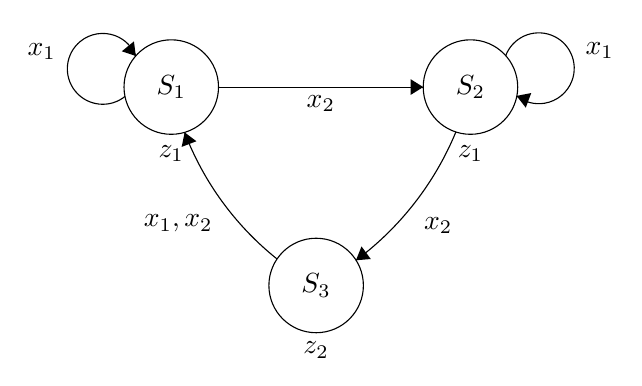
\begin{tikzpicture}[scale=0.2]
\tikzstyle{every node}+=[inner sep=0pt]
\draw [black] (16.9,-12.5) circle (3);
\draw (16.9,-12.5) node {$S_1$};
\draw (16.9,-16.7) node {$z_1$};
\draw [black] (35.9,-12.5) circle (3);
\draw (35.9,-12.5) node {$S_2$};
\draw (35.9,-16.7) node {$z_1$};
\draw [black] (26.1,-25.1) circle (3);
\draw (26.1,-25.1) node {$S_3$};
\draw (26.1,-29.2) node {$z_2$};
\draw [black] (19.9,-12.5) -- (32.9,-12.5);
\fill [black] (32.9,-12.5) -- (32.1,-12) -- (32.1,-13);
\draw (26.4,-13) node [below] {$x_2$};
\draw [black] (34.974,-15.35) arc (-22.43455:-53.31541:19.391);
\fill [black] (28.63,-23.5) -- (29.57,-23.42) -- (28.98,-22.62);
\draw (32.92,-21.27) node [right] {$x_2$};
\draw [black] (23.619,-23.419) arc (-128.64006:-159.08918:18.965);
\fill [black] (17.75,-15.38) -- (17.56,-16.3) -- (18.5,-15.94);
\draw (19.56,-21.17) node [left] {$x_1,x_2$};
\draw [black] (13.97,-13.089) arc (309.10321:21.10321:2.25);
\draw (9.61,-10.26) node [left] {$x_1$};
\fill [black] (14.65,-10.53) -- (14.53,-9.6) -- (13.76,-10.23);
\draw [black] (38.133,-10.515) arc (159.3696:-128.6304:2.25);
\draw (43.17,-10.18) node [right] {$x_1$};
\fill [black] (38.83,-13.06) -- (39.41,-13.81) -- (39.76,-12.88);
\end{tikzpicture}
\end{center}

%\begin{center}
%\begin{tikzpicture}[scale=0.2]
%\tikzstyle{every node}+=[inner sep=0pt]
%%\node[draw] at (0,0) {some text};
%\draw [black] (20.5,-17.8) circle (3);
%\draw (20.5,-17.8) node {$S_1$};
%\draw (20.5,-22) node {$z_1$};
%\draw [black] (39.7,-17.8) circle (3);
%\draw (39.7,-17.8) node {$S_2$};
%\draw (39.7,-22) node {$z_2$};
%\draw [black] (22.769,-15.848) arc (124.12588:55.87412:13.067);
%\fill [black] (37.43,-15.85) -- (37.05,-14.99) -- (36.49,-15.81);
%\draw (30.1,-13.1) node [above] {$x_2$};
%\draw [black] (37.402,-19.718) arc (-56.63019:-123.36981:13.275);
%\fill [black] (22.8,-19.72) -- (23.19,-20.58) -- (23.74,-19.74);
%\draw (30.1,-22.41) node [below] {$x_1$};
%\draw [black] (17.82,-19.123) arc (-36:-324:2.25);
%\draw (13.25,-17.8) node [left] {$x_1$};
%\fill [black] (17.82,-16.48) -- (17.47,-15.6) -- (16.88,-16.41);
%\draw [black] (42.38,-16.477) arc (144:-144:2.25);
%\draw (46.95,-17.8) node [right] {$x_2$};
%\fill [black] (42.38,-19.12) -- (42.73,-20) -- (43.32,-19.19);
%\draw [black] (42.38,-16.477) arc (144:-144:2.25);
%\fill [black] (42.38,-19.12) -- (42.73,-20) -- (43.32,-19.19);
%\end{tikzpicture}
%\end{center}

%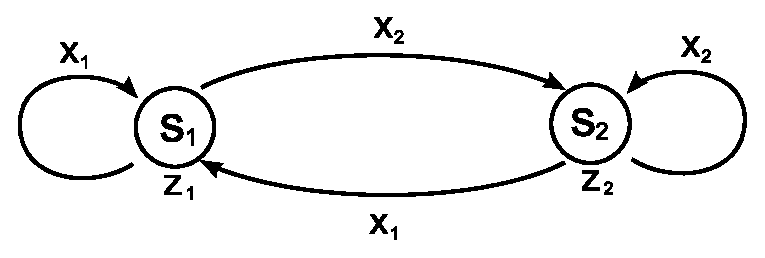
\includegraphics[width=0.5\linewidth]{slika_v9_2.eps}

\bigskip

Simulirajmo še delovanje avtomata pri vhodni besedi $x_1 x_1 x_2 x_2 x_2 x_2 x_1$ in začetnem stanju $S_1$ z uporabo spodnje tabele:

\bigskip

\begin{center}
\begin{tabular}{c|cccccccc}
vhodna črka 	&				& $x_1$ & $x_1$ & $x_2$ & $x_2$ & $x_2$ & $x_2$ & $x_1$ \\
\hline
stanje 				& $S_1$ & $S_1$ & $S_1$ & $S_2$ & $S_3$ & $S_1$ & $S_2$ & $S_2$ \\
\hline
izhodna črka	&				& $z_1$ & $z_1$ & $z_1$ & $z_2$ & $z_1$ & $z_1$ & $z_1$ 
\end{tabular}
\end{center}
\end{resitev}

\bigskip

Izhodna beseda je torej $z_1z_1z_1z_2z_1z_1z_1$.

\begin{zgled}
\label{Moore_door}
Nariši diagram prehajanja stanj in zapiši tabelo prehajanja stanj Moorovega avtomata, ki nadzira odpiranje krožnih vrat. Mehanizem drži vrata zaprta, dokler avtomat ne zazna, da je bil vstavljen kovanec. V tem primeru avtomat mehanizmu javi, da lahko sprosti zaporo vrat. Ko avtomat zazna prehod skozi vrata, ta javi mehanizmu, naj zapre vrata.
\end{zgled}

\begin{resitev}

Avtomat bo imel dve stanji, in sicer stanje, v katerem drži vrata zaprta ($S_1$) in ima tako izhodno črko $close$, in stanje, v katerem so vrata odprta ($S_2$) in ima tako izhodno črko $open$. Prehod iz $S_1$ v $S_2$ bomo izvedli, ko avtomat detektira, da je bil vstavljen kovanec (vhodna črka $coin$), prehod iz $S_2$ v $S_1$ pa, ko avtomat detektira prehod skozi vrata (vhodna črka $push$). 

\begin{center}
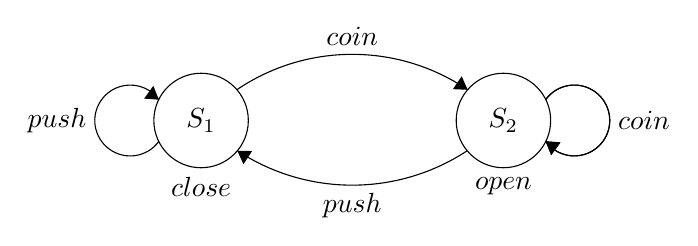
\begin{tikzpicture}[scale=0.2]
\tikzstyle{every node}+=[inner sep=0pt]
\draw [black] (20.5,-17.8) circle (3);
\draw (20.5,-17.8) node {$S_1$};
\draw (20.5,-22) node {$close$};
\draw [black] (39.7,-17.8) circle (3);
\draw (39.7,-17.8) node {$S_2$};
\draw (39.7,-22) node {$open$};
\draw [black] (22.769,-15.848) arc (124.12588:55.87412:13.067);
\fill [black] (37.43,-15.85) -- (37.05,-14.99) -- (36.49,-15.81);
\draw (30.1,-13.1) node [above] {$coin$};
\draw [black] (37.402,-19.718) arc (-56.63019:-123.36981:13.275);
\fill [black] (22.8,-19.72) -- (23.19,-20.58) -- (23.74,-19.74);
\draw (30.1,-22.41) node [below] {$push$};
\draw [black] (17.82,-19.123) arc (-36:-324:2.25);
\draw (13.25,-17.8) node [left] {$push$};
\fill [black] (17.82,-16.48) -- (17.47,-15.6) -- (16.88,-16.41);
\draw [black] (42.38,-16.477) arc (144:-144:2.25);
\draw (46.95,-17.8) node [right] {$coin$};
\fill [black] (42.38,-19.12) -- (42.73,-20) -- (43.32,-19.19);
\draw [black] (42.38,-16.477) arc (144:-144:2.25);
\fill [black] (42.38,-19.12) -- (42.73,-20) -- (43.32,-19.19);
\end{tikzpicture}
\end{center}

\bigskip

Zapišimo še tabelo prehajanja stanj avtomata:

\bigskip
\begin{center}
\begin{tabular}{c|cc}
&	$close$ & $open$\\
& $S_1$ & $S_2$\\
\hline
$coin$ & $S_2$ & $S_2$\\
$push$ & $S_1$ & $S_1$\\
\end{tabular}
\end{center}
\end{resitev}


\begin{zgled}
Za Mealyjev avtomat podan z diagramom prehajanja stanj zapiši tabelo prehajanja stanj. 

\bigskip

\begin{center}
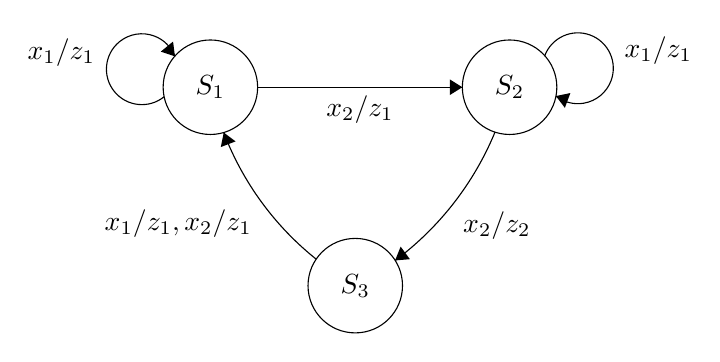
\begin{tikzpicture}[scale=0.2]
\tikzstyle{every node}+=[inner sep=0pt]
\draw [black] (16.9,-12.5) circle (3);
\draw (16.9,-12.5) node {$S_1$};
\draw [black] (35.9,-12.5) circle (3);
\draw (35.9,-12.5) node {$S_2$};
\draw [black] (26.1,-25.1) circle (3);
\draw (26.1,-25.1) node {$S_3$};
\draw [black] (19.9,-12.5) -- (32.9,-12.5);
\fill [black] (32.9,-12.5) -- (32.1,-12) -- (32.1,-13);
\draw (26.4,-13) node [below] {$x_2/z_1$};
\draw [black] (34.974,-15.35) arc (-22.43455:-53.31541:19.391);
\fill [black] (28.63,-23.5) -- (29.57,-23.42) -- (28.98,-22.62);
\draw (32.92,-21.27) node [right] {$x_2/z_2$};
\draw [black] (23.619,-23.419) arc (-128.64006:-159.08918:18.965);
\fill [black] (17.75,-15.38) -- (17.56,-16.3) -- (18.5,-15.94);
\draw (19.56,-21.17) node [left] {$x_1/z_1,x_2/z_1$};
\draw [black] (13.972,-13.097) arc (309.25644:21.25644:2.25);
\draw (9.61,-10.29) node [left] {$x_1/z_1$};
\fill [black] (14.65,-10.54) -- (14.53,-9.6) -- (13.75,-10.24);
\draw [black] (38.128,-10.509) arc (159.52411:-128.47589:2.25);
\draw (43.17,-10.15) node [right] {$x_1/z_1$};
\fill [black] (38.84,-13.06) -- (39.41,-13.81) -- (39.76,-12.87);
\end{tikzpicture}
\end{center}

\bigskip

Kakšno je zaporedje izhodnih črk (izhodna beseda), ki jo avtomat vrne pri zaporedju vhodnih črk (vhodni besedi) $x_1 x_1 x_2 x_2 x_2 x_2 x_1$ in začetnem stanju $S_1$?

\end{zgled}

\begin{resitev}

Abecede avtomata so enake kot pri Moorovem avtomatu iz zgleda \ref{Moore_basic}. Zapišimo tabelo prehajanja stanj:

\begin{center}
\begin{tabular}{c|ccc}
& $S_1$ & $S_2$ & $S_3$\\
\hline
$x_1$ & $S_1/z_1$ & $S_2/z_1$ & $S_1/z_1$\\
$x_2$ & $S_2/z_1$ & $S_3/z_2$ & $S_1/z_1$
\end{tabular}
\end{center}


\bigskip

Simulirajmo še delovanje avtomata pri vhodni besedi $x_1 x_1 x_2 x_2 x_2 x_2 x_1$ in začetnem stanju $S_1$ z uporabo spodnje tabele:

\bigskip

\begin{center}
\begin{tabular}{c|cccccccc}
vhodna črka 	&				& $x_1$ & $x_1$ & $x_2$ & $x_2$ & $x_2$ & $x_2$ & $x_1$ \\
\hline
stanje 				& $S_1$ & $S_1$ & $S_1$ & $S_2$ & $S_3$ & $S_1$ & $S_2$ & $S_2$ \\
\hline
izhodna črka	&				& $z_1$ & $z_1$ & $z_1$ & $z_2$ & $z_1$ & $z_1$ & $z_1$ 
\end{tabular}
\end{center}

\bigskip

Izhodna beseda je torej $z_1z_1z_1z_2z_1z_1z_1$.

\bigskip

Avtomat pri enakih pogojih generira enako izhodno abecedo kot Moorov avtomat iz zgleda \ref{Moore_basic}. Podrobnejša analiza bi pokazala, da sta si avtomata ekvivalentna.

\bigskip

\end{resitev}


\begin{zgled}
Nariši še Mealyjev avtomat v skladu z navodili iz zgleda \ref{Moore_door}.

%Mealyjev avtomat, ki kontrolira vklop in izklop luči.\\
%$X=\{push\}$\\
%$S=\{S_{on},S_{off}\}$\\
%$Z=\{Z_{on},Z_{off}\}$\\

%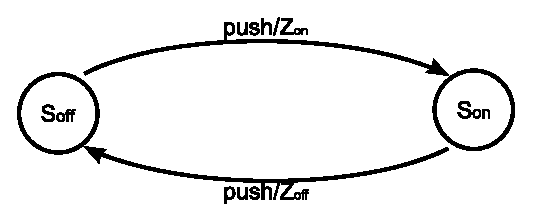
\includegraphics[width=0.5\linewidth]{slika_v9_luc_mealy.eps}

\end{zgled}

\begin{resitev}
V primeru Mealyjevega avtomata lahko avtomat z enim samim stanjem generira obe izhodni črki (\emph{open} in \emph{close}). Diagram prehajanja stanj ima tako sledečo obliko:

\begin{center}
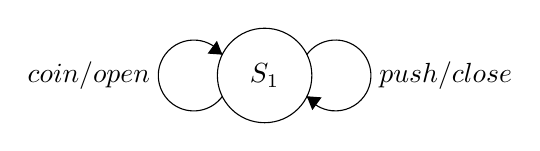
\begin{tikzpicture}[scale=0.2]
\tikzstyle{every node}+=[inner sep=0pt]
\draw [black] (23.5,-15.1) circle (3);
\draw (23.5,-15.1) node {$S_1$};
\draw [black] (26.18,-13.777) arc (144:-144:2.25);
\draw (30.75,-15.1) node [right] {$push/close$};
\fill [black] (26.18,-16.42) -- (26.53,-17.3) -- (27.12,-16.49);
\draw [black] (20.82,-16.423) arc (-36:-324:2.25);
\draw (16.25,-15.1) node [left] {$coin/open$};
\fill [black] (20.82,-13.78) -- (20.47,-12.9) -- (19.88,-13.71);
\end{tikzpicture}
\end{center}

Zapišimo še tabelo prehajanja stanj avtomata:

\begin{center}
\begin{tabular}{c|c}
& $S_1$ \\
\hline
$coin$ & $S_1/open$ \\
$push$ & $S_1/close$
\end{tabular}
\end{center}

\end{resitev}


%%
%%
%% Pretvorbe
%%
%%

\section{Pretvorbe med avtomati}

Kot smo videli že v prejšnjih zgledih imata lahko dva avtomata različnega tipa (Moore in Mealy) popolnoma enako delovanje in sta si tako ekvivalentna (izjema je začetna izhodna črka, saj Mealyjev avtomat le-to zgenerira šele pri prvem prehodu, pri Moorovem avtomatu pa je izhodna črka vedno prisotna). V splošnem velja, da za vsak Moorov avtomat obstaja vsaj en njegov Melyjev ekvivalent in obratno. 

Pretvorbo iz Melyjevega avtomata v Moorovega lahko izvedemo po sledečem postopku:
\begin{enumerate}
\item Mealyjev avtomat zapišemo tabelarično.
\item Zapišemo vse tri abecede Moorovega avtomata, pri čemer se vhodna in izhodna abecedi ohranjata, notranjo abeceda pa tvorimo s pari notranje stanje/izhodna črka, ki se pojavijo znotraj tabele Mealyjevega avtomata.
\item Zapišemo tabelo Moorovega avtomata, v kateri nastopajo vsa stanja, ki smo jih definirali v prejšnjem koraku. Izhodna črka za stanje je določena z izhodno črko, katere oznaka nastopa pri posameznem stanju. Prehodi med stanji so določeni s prehodi med ekvivalentimi stanji v Mealyjevem avtomatu,
\end{enumerate}

\begin{zgled}
Mealyjev avtomat, podan s spodnjim diagramom, pretvori v Moorov avtomat.

\begin{center}
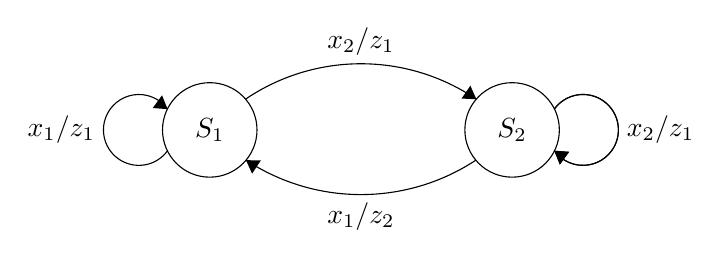
\begin{tikzpicture}[scale=0.2]
\tikzstyle{every node}+=[inner sep=0pt]
\draw [black] (20.5,-17.8) circle (3);
\draw (20.5,-17.8) node {$S_1$};
\draw [black] (39.7,-17.8) circle (3);
\draw (39.7,-17.8) node {$S_2$};
\draw [black] (22.769,-15.848) arc (124.12588:55.87412:13.067);
\fill [black] (37.43,-15.85) -- (37.05,-14.99) -- (36.49,-15.81);
\draw (30.1,-13.1) node [above] {$x_2/z_1$};
\draw [black] (37.402,-19.718) arc (-56.63019:-123.36981:13.275);
\fill [black] (22.8,-19.72) -- (23.19,-20.58) -- (23.74,-19.74);
\draw (30.1,-22.41) node [below] {$x_1/z_2$};
\draw [black] (17.82,-19.123) arc (-36:-324:2.25);
\draw (13.25,-17.8) node [left] {$x_1/z_1$};
\fill [black] (17.82,-16.48) -- (17.47,-15.6) -- (16.88,-16.41);
\draw [black] (42.38,-16.477) arc (144:-144:2.25);
\draw (46.95,-17.8) node [right] {$x_2/z_1$};
\fill [black] (42.38,-19.12) -- (42.73,-20) -- (43.32,-19.19);
\draw [black] (42.38,-16.477) arc (144:-144:2.25);
\fill [black] (42.38,-19.12) -- (42.73,-20) -- (43.32,-19.19);
\end{tikzpicture}
\end{center}

%\bigskip
%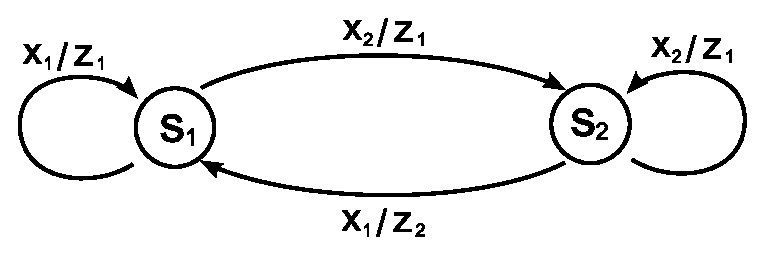
\includegraphics[width=0.5\linewidth]{slika_v9_3.eps}

\end{zgled}

\begin{resitev}

\bigskip
Podan Mealyjev avtomat zapišemo tabelarično:

\begin{center}
\begin{tabular}{c|cc}
 & $S_1$ & $S_2$\\
\hline
$x_1$ & $S_1/z_1$ & $S_1/z_2$\\
$x_2$ & $S_2/z_1$ & $S_2/z_1$
\end{tabular}
\end{center}

\bigskip
Notranjo abecedo Moorovega avtomata tvorijo pari naslednje stanje/izhodna črka Mealyjevega avtomata, ki se pojavijo znotraj tabele prehajanja stanj. Notranja abeceda je torej: $S_1/z_1$, $S_1/z_2$, $S_2/z_1$ (opomba: stanje $S_2/z_2$ lahko izpustimo, ker se v tabeli ne pojavi -- predpostavljamo, da to stanje ni začetno stanje avtomata). Zaradi lažjega zapisa stanja preimenujemo v: $S_{11}$, $S_{12}$, $S_{21}$. Vhodna in izhodna abeceda ostaneta enaki.

\bigskip
Na podlagi delovanja Melyjevega avtomata lahko tako zapišemo tabelo Moorovega avtomata:

\begin{center}
\begin{tabular}{c|ccc}
 & $z_1$ & $z_2$ & $z_1$\\
 & $S_{11}$ & $S_{12}$ & $S_{21}$\\
\hline
$x_1$ & $S_{11}$ & $S_{11}$ & $S_{12}$\\
$x_2$ & $S_{21}$ & $S_{21}$ & $S_{21}$
\end{tabular}
\end{center}
\bigskip
In ga narišemo.

%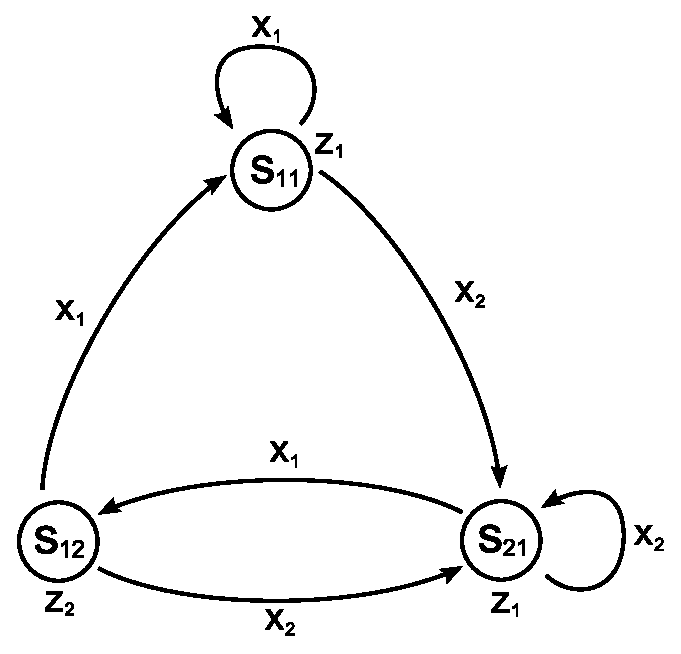
\includegraphics[width=0.4\linewidth]{slika_v9_4.eps}
\begin{center}
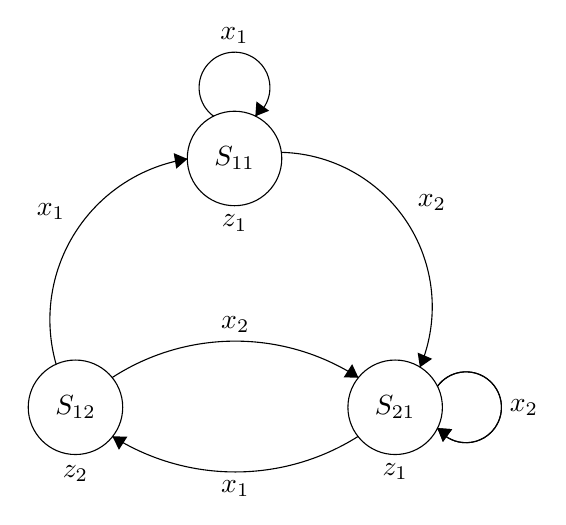
\begin{tikzpicture}[scale=0.2]
\tikzstyle{every node}+=[inner sep=0pt]
\draw [black] (19.5,-25.7) circle (3);
\draw (19.5,-25.7) node {$S_{12}$};
\draw (19.5,-29.9) node {$z_2$};
\draw [black] (39.8,-25.7) circle (3);
\draw (39.8,-25.7) node {$S_{21}$};
\draw (39.8,-29.8) node {$z_1$};
\draw [black] (29.6,-9.9) circle (3);
\draw (29.6,-9.9) node {$S_{11}$};
\draw (29.6,-14) node {$z_1$};
\draw [black] (21.827,-23.816) arc (123.00949:56.99051:14.359);
\fill [black] (37.47,-23.82) -- (37.07,-22.96) -- (36.53,-23.8);
\draw (29.65,-21) node [above] {$x_2$};
\draw [black] (37.446,-27.551) arc (-57.7201:-122.2799:14.597);
\fill [black] (21.85,-27.55) -- (22.26,-28.4) -- (22.8,-27.56);
\draw (29.65,-30.31) node [below] {$x_1$};
\draw [black] (42.48,-24.377) arc (144:-144:2.25);
\draw (47.05,-25.7) node [right] {$x_2$};
\fill [black] (42.48,-27.02) -- (42.83,-27.9) -- (43.42,-27.09);
\draw [black] (42.48,-24.377) arc (144:-144:2.25);
\fill [black] (42.48,-27.02) -- (42.83,-27.9) -- (43.42,-27.09);
\draw [black] (28.277,-7.22) arc (234:-54:2.25);
\draw (29.6,-2.65) node [above] {$x_1$};
\fill [black] (30.92,-7.22) -- (31.8,-6.87) -- (30.99,-6.28);
\draw [black] (18.272,-22.974) arc (-164.06157:-261.11516:10.332);
\fill [black] (26.61,-9.93) -- (25.74,-9.56) -- (25.9,-10.55);
\draw (18.88,-13.26) node [left] {$x_1$};
\draw [black] (32.563,-9.511) arc (88.71632:-23.0262:9.813);
\fill [black] (41.37,-23.16) -- (42.15,-22.62) -- (41.23,-22.23);
\draw (41.21,-12.68) node [right] {$x_2$};
\end{tikzpicture}
\end{center}

\bigskip
\end{resitev}

Po podobnem postopku lahko izvedemo pretvorbo Moorovega v Mealyjev avtomat:
\begin{enumerate}
\item Moorov avtomat zapišemo tabelarično.
\item Zapišemo vse tri abecede Mealyjevega avtomata, ki so kar enake abecedam Moorovega avtomata.
\item Zapišemo tabelo Mealyjevega avtomata, pri čemer je naslednje stanje enako kot pri Moorovem avtomatu, izhodna črka pa je določena z izhodno črko stanja Moorovega avtomata, v katerega bo avtomat z določeno kombinacijo stanje/vhodna črka prišel.
\end{enumerate}



\begin{zgled}

Moorov avtomat, ki predstavlja rešitev prejšnjega zgleda, pretvori v Mealyjev avtomat.

\end{zgled}

\begin{resitev}

Pretvorimo dobljeni Moorov avtomat nazaj v Mealyjevega. Vse tri abecede se ohranjajo. Zapišimo tabelo prehajanja stanj:

\begin{center}
\begin{tabular}{c|ccc}
 & $S_{11}$ & $S_{12}$ & $S_{21}$\\
\hline
$x_1$ & $S_{11}/z_1$ & $S_{11}/z_1$ & $S_{12}/z_2$\\
$x_2$ & $S_{21}/z_1$ & $S_{21}/z_1$ & $S_{21}/z_1$
\end{tabular}
\end{center}


Dobili smo avtomat s tremi notranji stanji, ki je enakovreden prvotnemu Mealyjevemu avtomatu z dvema stanjema. Stanji $S_{11}$ in $S_{12}$ sta enaki tako po izhodnih črkah kot tudi po prehodih. Stanji lahko tako zakodiramo zgolj z enim notranjim stanjem -- recimo mu stanje $S_1$. Stanje $S_{21}$ preimenujmo, da bo zapis avtomata bolj pregleden -- recimo mu stanje $S_2$. Nad stanji avtomata tako izvedemo sledečo preslikavo:
$S_{11} \rightarrow S_1$\\
$S_{12} \rightarrow S_1$\\
$S_{21} \rightarrow S_2$\\

\bigskip

Tako dobimo avtomat, ki je enak izhodiščnemu:

\begin{center}
\begin{tabular}{c|cc}
 & $S_1$ & $S_2$\\
\hline
$x_1$ & $S_1/z_1$ & $S_1/z_2$\\
$x_2$ & $S_2/z_1$ & $S_2/z_1$
\end{tabular}
\end{center}

\bigskip

\end{resitev}